\section{Multiple Dot Products (4 Points total)}
\subsection{Task 2a}
In this Section it was asked specifically to "write a Kernel", so that is what you will find below, just a Kernel without any useful implementation!

\begin{lstlisting}[language=C++, title=C++ Cuda Code Kernel for 2a]
__global__ void cuda_2a(int N, double *x, double *y, double *result)
{
  __shared__ double shared_m1[256];
  __shared__ double shared_m2[256];
  __shared__ double shared_m3[256];
  __shared__ double shared_m4[256];
  __shared__ double shared_m5[256];
  __shared__ double shared_m6[256];
  __shared__ double shared_m7[256];
  __shared__ double shared_m8[256];
 
  double dot1=0, dot2=0, dot3=0, dot4=0, dot5=0, dot6=0, dot7=0, dot8=0;
  for (int i = blockIdx.x * blockDim.x + threadIdx.x; i < N; i += blockDim.x * gridDim.x) {
    dot1 += x[i] * y[i];
    dot2 += x[i] * y[i+N];
    dot3 += x[i] * y[i+2*N];
    dot4 += x[i] * y[i+3*N];
    dot5 += x[i] * y[i+4*N];
    dot6 += x[i] * y[i+5*N];
    dot7 += x[i] * y[i+6*N];
    dot8 += x[i] * y[i+7*N];
  }
 
  shared_m1[threadIdx.x] = dot1;
  shared_m2[threadIdx.x] = dot2;
  shared_m3[threadIdx.x] = dot3;
  shared_m4[threadIdx.x] = dot4;
  shared_m5[threadIdx.x] = dot5;
  shared_m6[threadIdx.x] = dot6;
  shared_m7[threadIdx.x] = dot7;
  shared_m8[threadIdx.x] = dot8;

  for (int k = blockDim.x / 2; k > 0; k /= 2) {
    __syncthreads();
    if (threadIdx.x < k) {
      shared_m1[threadIdx.x] += shared_m1[threadIdx.x + k];
      shared_m2[threadIdx.x] += shared_m2[threadIdx.x + k];
      shared_m3[threadIdx.x] += shared_m3[threadIdx.x + k];
      shared_m4[threadIdx.x] += shared_m4[threadIdx.x + k];
      shared_m5[threadIdx.x] += shared_m5[threadIdx.x + k];
      shared_m6[threadIdx.x] += shared_m6[threadIdx.x + k];
      shared_m7[threadIdx.x] += shared_m7[threadIdx.x + k];
      shared_m8[threadIdx.x] += shared_m8[threadIdx.x + k];
    }
  }
 
  if (threadIdx.x == 0){
    atomicAdd(&result[0], shared_m1[0]);
    atomicAdd(&result[1], shared_m2[0]);
    atomicAdd(&result[2], shared_m3[0]);
    atomicAdd(&result[3], shared_m4[0]);
    atomicAdd(&result[4], shared_m5[0]);
    atomicAdd(&result[5], shared_m6[0]);
    atomicAdd(&result[6], shared_m7[0]);
    atomicAdd(&result[7], shared_m8[0]);
  }
}
\end{lstlisting}

\pagebreak

\subsection{Task 2b}
"Add a loop around that kernel to call it K/8 times to correctly compute the K dot products"
This was achieved by adjusting the algorithm in the following way:

\begin{lstlisting}[language=C++, title=C++ Cuda Code adaptation 2b]
void Loop_function(int N, int K, double *x, double **y, double **results)
{
    int h= K/8;
    for (; h>0; h--)
    {
        cuda_task2<<<256, 256>>>(N, x, y[h-1], results[h-1]);
    }
}

float avg_vec(std::vector<float> timings_vec)
{
    float avg = std::accumulate(timings_vec.begin(), timings_vec.end(), 0.0);
    avg /= timings_vec.size();
    return avg;
}

int main(void)
{

  Timer timer;

  for (int N = 1000; N < 1000001; N *= 10)
  {
      for (size_t K = 8; K < 33; K += 8)
      {

      std::vector<float> timings;

      //
      // allocate host memory:
      //
      
      double *x = (double*)malloc(sizeof(double) * N);
      double *results  = (double*)malloc(sizeof(double) * K);
      double **results3 = (double**)malloc(sizeof(double) * K/8);
      for (size_t i=0; i<K/8; ++i) {
        results3[i] = (double*)malloc(sizeof(double) * 8);
      }

      double **v = (double**)malloc(sizeof(double*) * K/8);
      for (size_t i=0; i<K/8; ++i) {
        v[i] = (double*)malloc(sizeof(double) * N*8);
      }

      //
      // allocate device memory
      //

      double *cuda_x; cudaMalloc((&cuda_x), sizeof(double)*N);
      double **cuda_v = (double**)malloc(sizeof(double*) * K/8);  
      for (size_t i=0; i<K/8; ++i) {
        cudaMalloc( (void **)(&cuda_v[i]), sizeof(double)*N*8);
      }

      double **cuda_results3 = (double**)malloc(sizeof(double*) * K/8); 
      for (size_t i=0; i<K/8; ++i) {
        cudaMalloc( (void **)(&cuda_results3[i]), sizeof(double)*8);
      }
    
      //
      // initialize v
      //

      std::fill(x, x + N, 1.0);
      for (size_t i=0; i<K/8; ++i) {
        for (size_t j=0; j<N*8; ++j) {
          v[i][j] = 1 + rand() / (1.1 * RAND_MAX);
        }
      }

      //
      // Reference calculation on CPU:
      //

      for (size_t i=0; i<K; ++i) {results[i]=0;}
      // dot product
      for (size_t i=0; i<K/8; ++i) {
        for (size_t j=0; j<N*8; ++j) {
          results[i*8+j/N] += x[j%N] * v[i][j];
        }
      }
      
      //
      // Copy data to GPU
      //
      
      cudaMemcpy(cuda_x, x, sizeof(double)*N, cudaMemcpyHostToDevice);
      for (size_t i=0; i<K/8; ++i) {
        cudaMemcpy(cuda_v[i], v[i], sizeof(double)*N*8, cudaMemcpyHostToDevice);
      }

      for (int i = 0; i < 11; i++)
      {
        //
        // CUDA implementation
        //

        CUDA_ERRCHK(cudaDeviceSynchronize());
        timer.reset(); 
        Loop_function(N, K, cuda_x, cuda_v, cuda_results3);
        CUDA_ERRCHK(cudaDeviceSynchronize());
        float elapsed_time_0 = timer.get();
        if (i > 0)
        {
            timings.push_back(elapsed_time_0);
        }

      }

      std::cout << N << "," << K << "," << avg_vec(timings) << std::endl;

      //
      // Copy data to Host
      //

      for (size_t i=0; i<K/8; ++i) {
        cudaMemcpy(results3[i], cuda_results3[i], sizeof(double)*8, cudaMemcpyDeviceToHost);
      }
\end{lstlisting}

\pagebreak

\subsection{Task 2c}

In figure 1 below, the plot for task 2c.

\begin{figure}[h]
    \begin{center}
        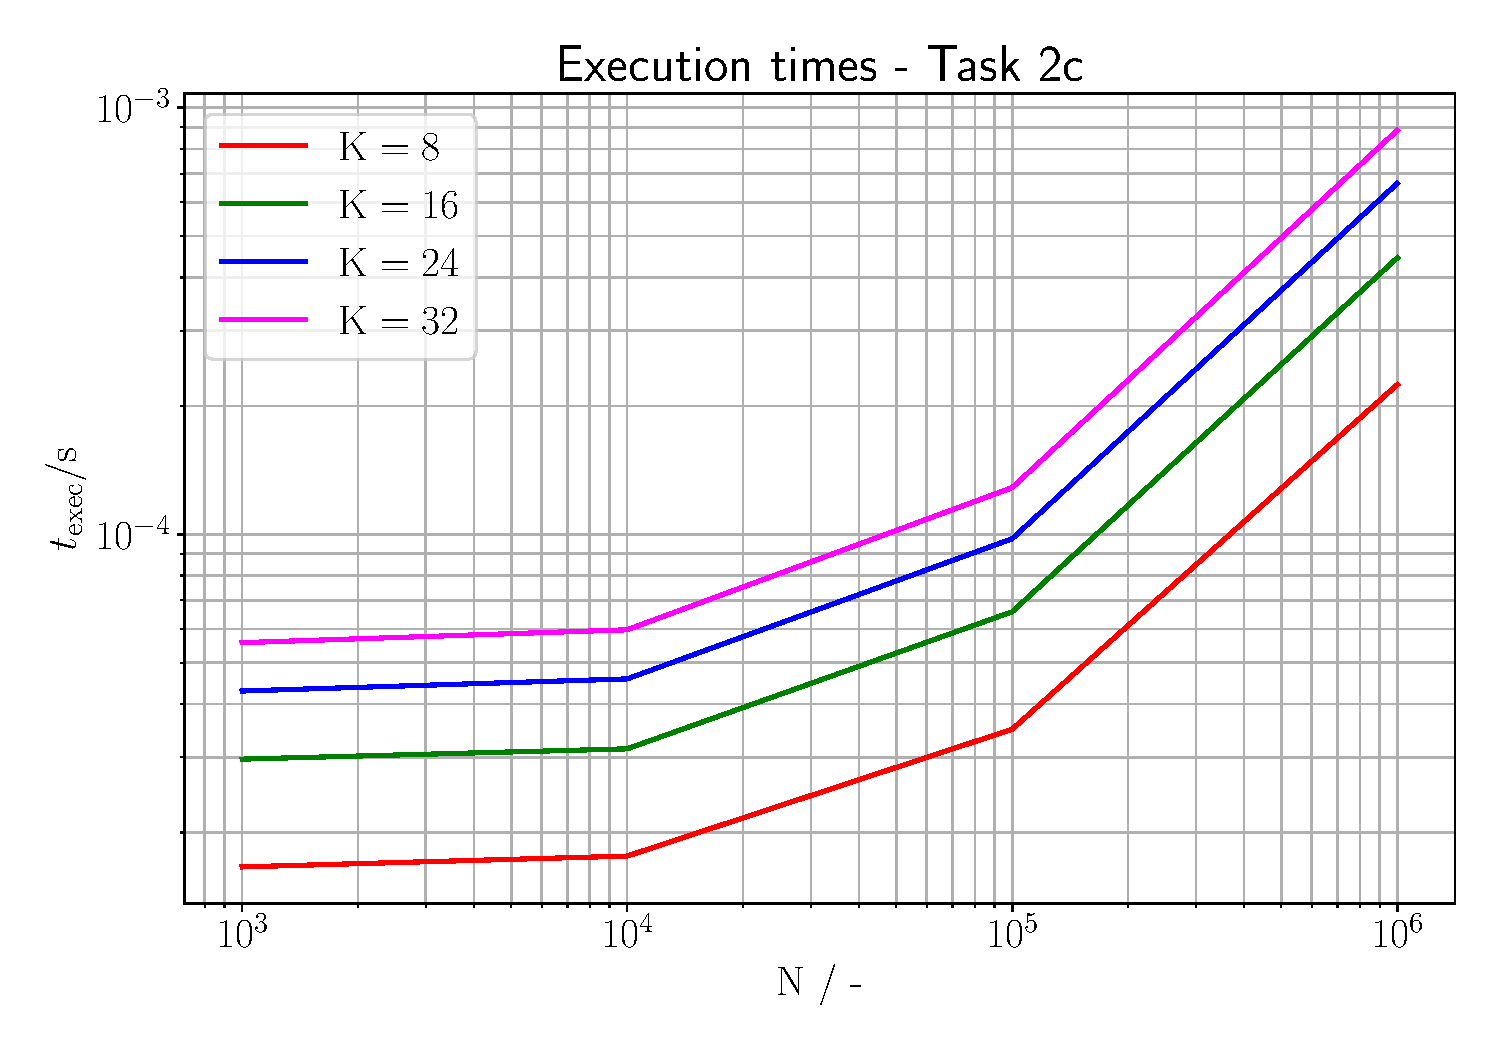
\includegraphics[width=15cm]{figures/task_2_c.pdf}
        \caption{Execution Times of concurrent dot products for different $\mathrm{K}$ and $\mathrm{N}$}
    \end{center}
\end{figure}

\subsection{Task 2d}

By checking if k mod(8) is 0, if not find a scheme to additionally start another kernel for a single dot product to balance out, otherwise 
proceed as before.